\chapter{Revisão bibliográfica} \label{chap:revBibli}
	\section{Breve revisão dos conceitos utilizados neste trabalho}

		\subsection{Sinais digitais e sub-amostragem (\textit{downsampling})}
			\par Os sinais de voz digitais, isto é, aqueles que estão amostrados e quantizados \cite{haykin2011sistemas}, constituem a base deste trabalho. Além do processo de digitalização, inerente ao ato de armazenar locuções em computadores, os sinais podem sofrer, a depender da necessidade ou possibilidade, sub-amostragens ou \textit{downsamplings} \cite{robi2003}. Isso implica a estratégia de redução de dimensão e, comumente, ocorre após a conversão de domínio dos sinais com base em filtros digitais do tipo \textit{wavelet}, a serem apresentados adiante. Um exemplo consta na Figura \ref{fig:downsampling}, na qual as partes pretas contêm dados e as brancas representam os elementos removidos. Tendo em vista que este trabalho está baseado em sinais digitais de voz filtrados com base em \textit{wavelets}, o processo de sub-amostragem é essencial. 
			\begin{figure}[h]
				\centering
				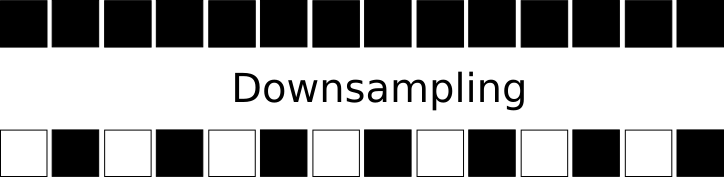
\includegraphics[width=0.7\linewidth]{images/downsampling}
				\caption{Sub-amostragem}
				\label{fig:downsampling}
			\end{figure}
			
		\subsection{Caracterização dos processos de produção da voz humana}
			\par A fala possui três grandes áreas de estudo: A fisiológica, também conhecida como fonética articulatória, a acústica, referida como fonética acústica, e ainda, a perceptual, que cuida da percepção  da  fala \cite{kremer2014eficiencia}. Neste trabalho, o foco será apenas na questão acústica, pois não serão analisados aspectos da fisiologia relacionada à voz, mas sim os sinais sonoros propriamente ditos.
			
			\subsubsection{Sinais vozeados \textit{versus} não-vozeados}

			\par Quando da análise dos sinais de voz, consideram-se as partes vozeadas e não-vozeadas. Aquelas são produzidas com a ajuda da vibração quase periódica das pregas vocais, enquanto estas praticamente não contam com participação regrada da referida estrutura.
			
			\subsubsection{Frequência fundamental da voz}
				\par Também conhecida como $F_0$, é o componente periódico resultante da vibração das pregas vocais. Em termos de percepção, se pode interpretar $F_0$ como o tom da voz, isto é, a frequência de \textit{pitch} \cite{kremer2014eficiencia}. Vozes agudas tem uma frequência de \textit{pitch} alto, enquanto vozes mais graves tem baixa. A alteração da frequência (jitter) e/ou intensidade (shimmer) do \textit{pitch} durante a fala é definida como entonação,  porém, também pode indicar algum distúrbio ou doença relacionada ao trato vocal \cite{WERTZNER2005}.
				
				\par A frequência fundamental da voz é o número de vezes na qual uma forma de onda característica, que reflete a excitação pulmonar moldada pelas pregas vocais, se repete por unidade de tempo. Sendo assim, as medidas de $F_0$ geralmente são apresentadas em Hz \cite{freitas2013avaliaccao}.
			
				\par A medição de $F_0$ está sujeita a contaminações surgidas das variações naturais de \textit{pitch} típicas da voz humana \cite{freitas2013avaliaccao}. A importância de se medir $F_0$ corretamente vem do fato de que, além de carregar boa parte da informação da fala, ela é a base para construção das outras frequências que compõe os sinais de voz, que são múltiplas de $F_0$.
				
				\subsubsection{Formantes}
					\par O sinal de excitação que atravessa as pregas vocais é rico em harmônicas, isto é, frequências múltiplas da fundamental. Tais harmônicas podem ser atenuadas ou amplificadas, em função da estrutura dos tratos vocal e nasal de cada locutor. Particularmente, o primeiro formante ($F_1$), relaciona-se à  amplificação  sonora  na  cavidade  oral  posterior  e  à  posição  da  língua  no  plano  vertical;  o segundo  formante  ($F_2$)  à  cavidade  oral  anterior  e  à  posição  da  língua  no  plano  horizontal; o terceiro  formante  ($F_3$)  relaciona-se  às  cavidades  à  frente  e  atrás  do  ápice  da  língua e, finalmente,  o  quarto formante  ($F_4$) relaciona-se  ao  formato  da  laringe  e  da  faringe  na  mesma  altura  \cite{valencca2014analise}. Formantes caracterizam fortemente os locutores, pois cada indivíduo possui um formato de trato vocal e nasal. Assim, tais frequências, que podem ser capturadas com ferramentas diversas, a exemplo da Transformada \textit{Wavelet}, são de suma importância na área de verificação de locutores.

\subsection{Distâncias Euclidiana e Manhattan}
    \par Por definição, as distâncias Euclidiana ($D_E$) e Manhattan ($D_M$) entre dois vetores $x[\cdot]$ e $y[\cdot]$ de tamanho $M$ são dadas, respectivamente, por:
    \begin{equation}
     D_E = \sqrt{\sum\limits_{i=0}^{M-1}(x_i - y_i)^2}
    \end{equation}
	e
    \begin{equation}
        D_M = \sqrt{\sum\limits_{i=0}^{M-1}|x_i - y_i|}   
        \qquad. 
    \end{equation}

\subsection{Escalas e energias dos sinais}
	\par A energia de um sinal digital $s[\cdot]$ com $M$ amostras é definida como
	\begin{equation}
	E = \sum\limits_{i=0}^{M-1}(s_i)^2 \qquad.   
	\end{equation}
	$E$ pode ainda sofrer normalizações e ter a sua mensuração restrita a uma parte específica do sinal sob análise. Possibilidades para tais restrições podem, por exemplo, envolver a escala BARK \cite{doi:10.1121-1.1908630} e MEL \cite{beranek1949acoustic} que serão utilizadas neste trabalho.
	\subsubsection{A escala BARK}
		\par BARK foi definida tendo em mente vários tipos de sinais acústicos. Essa escala corresponde ao conjunto de 25 bandas críticas da audição humana. Suas frequências-base de audiometria são, em Hz: \textbf{20, 100, 200, 300, 400, 510, 630, 770, 920, 1080, 1270, 1480, 1720, 2000, 2320, 2700, 3150, 3700, 4400, 5300, 6400, 7700, 9500, 12000, 15500}. Nessa escala,os sinais digitais no domínio temporal atravessam filtros passa-faixas \cite{bosi2002introduction} para os quais o início e o final da banda de passagem correspondem à frequências-base consecutivas resultando em um vetor de características com 24 coeficientes e, em seguida, as energias dos sinais filtrados são utilizadas como características descritivas de propriedades do sinal sob análise, como mostrado na Figura \ref{fig:barkfeaturevect}.
		\begin{figure}[h]
			\centering
			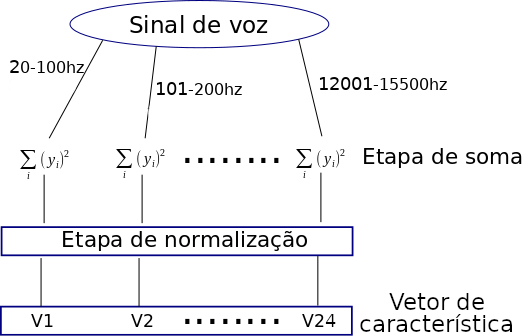
\includegraphics[width=0.6\linewidth]{images/barkFeatureVect}
			\caption{Cálculo de vetores de características com BARK}
			\label{fig:barkfeaturevect}
		\end{figure}
	\subsubsection{A escala MEL}
		\par Escala Mel, advinda do termo \textit{melody}, é uma adaptação da escala Bark para sinais de voz. Dentre as várias implementações de bandas críticas a escolhida foi a implementação que contém os valores em Hz: \textbf{20, 160, 394, 670, 1000, 1420, 1900, 2450, 3120, 4000, 5100, 6600, 9000, 14000}.
		\par A variante que será usada neste trabalho é conhecida como \textit{Mel-frequency cepstral coefficients}(MFCC) a qual inclui, além dos intervalos definidos, uma diminuição da correlação entre os componentes gerados via aplicação da Transformada Discreta Cosseno (DCT) \cite{salomon2007data} ou da Análise de Componentes Principais (PCA) \cite{jolliffe2006principal} seguida de duas derivações no vetor de características resultando em um total de 11 coeficientes. Nesse trabalho foi escolhida a DCT, no entanto, PCA poderia também ser escolhida sem prejuízos, o uso de uma ou outra depende da preferência do autor.
		\par Novamente, desconsiderando qualquer etapa intermediária que possa ser adicionada, as energias calculadas nos intervalos definidos na escala MEL podem, por si mesmas, constituir um vetor de características, como mostrado na Figura \ref{fig:barkfeaturevect}.
		\begin{figure}[h]
			\centering
			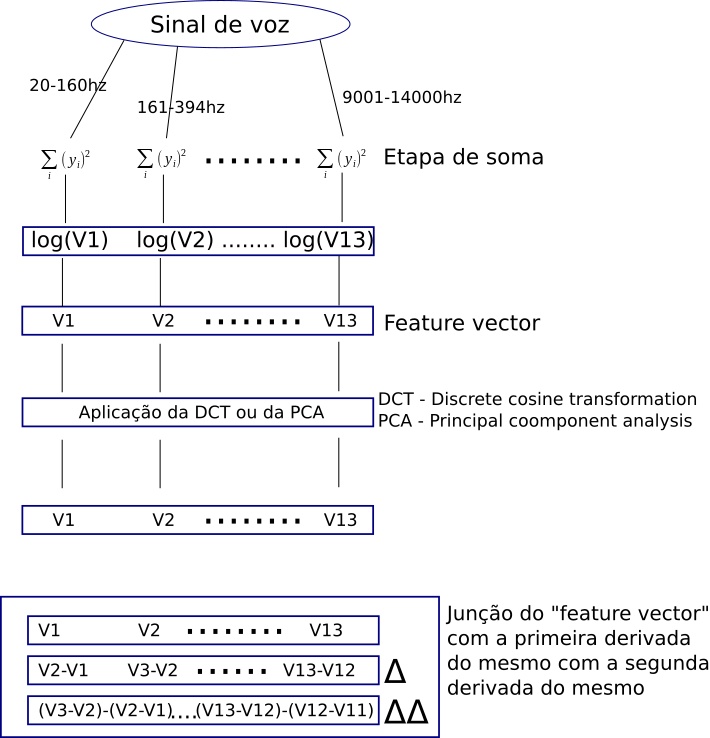
\includegraphics[width=0.8\linewidth]{images/melFeatureVect}
			\caption{Cálculo de vetores de características com MEL}
			\label{fig:melfeaturevect}
		\end{figure}
	
		\subsection{Filtros digitais \textit{wavelet}}
			\par Filtros digitais \textit{wavelet} têm sido utilizados com sucesso para suprir as deficiências de janelamento de sinal apresentadas pelas Transformadas de Fourier e de Fourier de Tempo Reduzido. \textit{Wavelets} contam com variadas funções-filtro e têm tamanho de janela variável, o que permite uma análise multirresolução \cite{Rod5254905}. Particularmente, as \textit{wavelets} proporcionam a análise do sinal de forma detalhada tanto no espectro de baixa frequência quanto no de alta contando com diferentes funções-base não periódicas diferentemente da tradicional transformada de Fourrier que utilizam somente as bases periódicas senoidal e cossenoidal.
			
			\par É importante observar que, quando se trata de Transformadas \textit{Wavelet}, seis elementos estão presentes: dois filtros de análise, dois filtros de síntese e as funções ortogonais \textit{scaling} e \textit{wavelet}. No tocante a sua aplicação, só a transformada direta, e não a inversa, será usada na construção dos vetores de características. Portanto, os filtros de síntese, a função \textit{scaling} e a função \textit{wavelet} não serão elementos abordados aqui: eles somente interessariam caso houvesse a necessidade da transformada inversa.

			\par No contexto dos filtros digitais baseados em \textit{wavelets}, o tamanho da janela recebe o nome de \textbf{suporte}. Janelas definem o tamanho do filtro que será aplicado ao sinal. Quando esse é pequeno (limitado), se diz que a janela tem \textbf{um suporte compacto} \cite{robi2003}.
		
			\par Se diz que uma \textit{wavelet} tem boa \textbf{resposta em frequência} quando, na aplicação da mesma para filtragem, não são causadas muitas pertubações indesejadas ao sinal, no domínio da frequência. Os filtros \textit{wavelet} de Daubechies \cite{daubechies1992ten} se destacam nesse quesito por serem \textit{maximamente planos} (\textit{maximally-flat}) \cite{butterworth1930} \cite{bianchi2007electronic} nos platôs de resposta em frequência como indicado na Figura \ref{fig:daubechies} ao contrário do que ocorre na Figura \ref{fig:nomaximallyflat}.

			\begin{figure}[h]
				\centering
				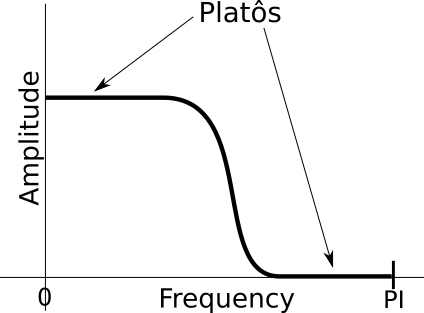
\includegraphics[width=0.3\linewidth]{images/daubechies}
				\caption{Platôs maximamente planos em um filtro digital: característica da família de Daubechies}
				\label{fig:daubechies}
			\end{figure}

			\begin{figure}[h]
				\centering
				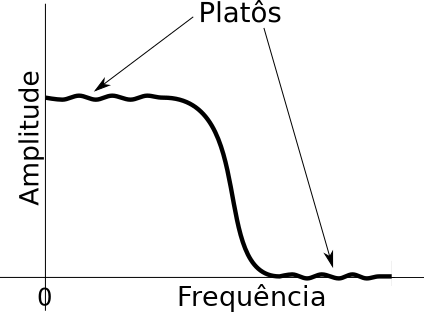
\includegraphics[width=0.3\linewidth]{images/noMaximallyFlat}
				\caption{Platôs não maximamente planos de um filtro digital: características de outros filtros \textit{wavelet}, distintos da família de Daubechies}
				\label{fig:nomaximallyflat}
			\end{figure}
		
			\par Além da resposta em frequência, na aplicação de um filtro digital \textit{wavelet} também é possível considerar a \textbf{resposta em fase}, que constitui um atraso ou adiantamento do sinal filtrado em relação ao sinal original, ambos no domínio temporal. Esse deslocamento pode ser \textbf{linear}, \textbf{quase linear} ou \textbf{não linear}: 
			
			\begin{itemize}
				\item na resposta em fase \textbf{linear}, há o mesmo deslocamento de fase para todos os componentes do sinal;
				\item quando a resposta em fase é \textbf{quase linear} existe uma pequena diferença no deslocamento dos diferentes componentes do sinal;
				\item finalmente, quando a resposta é \textbf{não linear}, acontece um deslocamento significativamente heterogêneo para as diferentes frequências que compõe o sinal.
				\end{itemize}
			
			\par Idealmente, é desejável que todo filtro apresente boa resposta em frequência e em fase linear. Características de fase e frequência de algumas famílias de filtros \textit{wavelet} constam na Tabela \ref{tab:waveletsProperties}.
			
			\begin{table}[h]
	\centering
	\caption{Algumas das \textit{wavelets} mais usadas e suas propriedades}
	\begin{tabular}{|c|p{75mm}|c|}
			\hline 
			\textbf{Wavelet} & \textbf{Resposta em frequência} & \textbf{Resposta em fase} \\ 
			\hline 
			Haar & Pobre &  Linear \\ 
			\hline 
			Daubechies & mais próxima da ideal à medida que o \newline  suporte aumenta; \textit{maximally-flat}  &  Não linear \\ 
			\hline 
			Symmlets & mais próxima da ideal à medida que o \newline  suporte aumenta; não \textit{maximally-flat}  & Quase linear \\ 
			\hline 
			Coiflets & mais próxima da ideal à medida que o \newline  suporte aumenta; não \textit{maximally-flat}  & Quase linear \\ 
			\hline 
	\end{tabular} 
	\label{tab:waveletsProperties}
	\\Fonte: Elaborado pelo autor, 2021.
\end{table}


		\subsubsection{O algoritmo de Mallat para a Transformada \textit{Wavelet}}
			\par Baseando-se no artigo \citetext{7079589}, percebe-se que algoritmo de Mallat faz com que aplicação das \textit{wavelets} seja uma simples multiplicação de matrizes. O sinal que deve ser transformado se torna uma matriz linear vertical. Os filtros passa-baixa e passa-alta tornam-se, nessa ordem, linhas de uma matriz quadrada que será completada segundo regras que serão mostradas mais adiante. É importante que essa matriz quadrada tenha a mesma dimensão que o sinal a ser transformado.
		
			\par Interessantemente, para que seja possível a transformação \textit{wavelet}, basta ter disponível o vetor do filtro passa-baixas calculado a partir da \textit{mother wavelet}, que é a função geradora desse filtro, já que o passa-alta pode ser construído a partindo-se da ortogonalidade do primeiro.
			
			\par Determinar a ortogonal de um vetor significa construir um vetor, tal que, o produto escalar do vetor original com sua respectiva ortogonal seja nulo.
			
			\par Considerando $h[\cdot]$ como sendo o vetor do filtro passa-baixas e $g[\cdot]$ seu correspondente ortogonal, tem-se que $h[\cdot] \cdot g[\cdot] = 0 \qquad .$
			\par Portanto, se $h[\cdot]=[a, b, c, d]$ então seu ortogonal será $g[\cdot]=[d, -c, b, -a]$ pois:
			$$
				h[\cdot] \cdot g[\cdot]  =  [a, b, c, d] \cdot [d, -c, b, -a] = (a \cdot d) + (b \cdot (-c)) + (c \cdot b) + (d \cdot (-a)) = ad - ad + bc - bc = 0 \qquad.
			$$

			\par A título de exemplo, considera-se:
			\begin{itemize}
				\item o filtro passa baixa baseado na \textit{wavelet} Haar: $h[\cdot] = [\frac{1}{\sqrt{2}}, \frac{1}{\sqrt{2}}]$
				\item o seu respectivo vetor ortogonal: $g[\cdot] = [\frac{1}{\sqrt{2}}, \frac{-1}{\sqrt{2}}]$
				\item e também o seguinte sinal-exemplo de entrada: $s = \{1,2,3,4\}$
			\end{itemize}

			\par Se o tamanho do sinal a ser tratado é quatro e se pretende-se aplicar o filtro Haar, a seguinte matriz de coeficientes é construída:
			\begin{equation}
				\begin{pmatrix}
					\frac{1}{\sqrt{2}}, \frac{1}{\sqrt{2}}, 0, 0\\
					\frac{1}{\sqrt{2}}, \frac{-1}{\sqrt{2}}, 0, 0\\
					0, 0, \frac{1}{\sqrt{2}}, \frac{1}{\sqrt{2}}\\
					0, 0, \frac{1}{\sqrt{2}}, \frac{1}{\sqrt{2}}
					\label{eq:haarFilters}
				\end{pmatrix} 
			\end{equation}
			\par Tendo em vista que a dimensão do sinal sob análise é diferente da dimensão do filtro, basta completar cada uma das linhas da matriz de coeficientes com zeros. A matriz é montada de forma que ela seja ortogonal.

			\par Montada a matriz de filtros, segue-se com os cálculos da transformada:
			\begin{equation}
				\begin{pmatrix}
					\frac{1}{\sqrt{2}}, \frac{1}{\sqrt{2}}, 0, 0\\
					\frac{1}{\sqrt{2}}, \frac{-1}{\sqrt{2}}, 0, 0\\
					0, 0, \frac{1}{\sqrt{2}}, \frac{1}{\sqrt{2}}\\
					0, 0, \frac{1}{\sqrt{2}}, \frac{1}{\sqrt{2}}\\
				\end{pmatrix} 
				\cdot
				\begin{pmatrix}
					1\\
					2\\
					3\\
					4\\
				\end{pmatrix} 
				=
				\begin{pmatrix}
					\frac{3}{\sqrt{2}}\\
					\frac{-1}{\sqrt{2}}\\
					\frac{7}{\sqrt{2}}\\
					\frac{-1}{\sqrt{2}}
				\end{pmatrix}
				\label{eq:haarMultiplic}
			\end{equation}
			
			\par Realizada a multiplicação, é necessário montar o sinal filtrado. Isso é feito escolhendo, dentro do resultado, valores alternadamente de forma que o vetor resultante seja:

			\begin{equation}
				resultado = \Big[
				\frac{3}{\sqrt{2}},
				\frac{7}{\sqrt{2}},
				\frac{-1}{\sqrt{2}},
				\frac{-1}{\sqrt{2}}
				\Big]\qquad.
				\label{eq:haarResult}
			\end{equation}
			
			\par Percebe-se que, na transformação descrita nas Equações \ref{eq:haarFilters}, \ref{eq:haarMultiplic} e \ref{eq:haarResult}, a \textbf{aplicação dos filtros sobre o vetor de entrada ocorreu apenas uma vez}. Sendo assim, se diz que o sinal recebeu uma \textbf{transformação de nível 1}. A cada transformação, há uma separação do sinal em dois componentes: o de baixa e o de alta frequência.
			
			\par Embora haja um limite, que será mencionado adiante, é possível aplicar mais de um nível de decomposição ao sinal. Para que se possa fazer isso, a Transformada \textit{Wavelet} nível 2 deve considerar apenas a parte de baixas frequências da primeira transformada; a transformada de nível 3 deve considerar apenas a parte de baixas frequências da transformada nível 2, e assim consecutivamente.
			
			\par Nos exemplos numéricos mostrados nas Tabelas \ref{tab:regularWaveletExample}, \ref{tab:packetWaveletExampleLF} e \ref{tab:packetWaveletExampleHF}, usou-se um filtro normalizado cujos coeficientes são $\{\dfrac{1}{2},-\dfrac{1}{2}\}$. Os dados destacados em \textbf{verde} correspondem ao \textbf{vetor original} que será tratado. Cada uma das linhas são os resultados das transformações nos níveis 1, 2, 3 e 4, respectivamente. As partes em \textbf{azul} correspondem à porção de \textbf{baixas frequências}, enquanto que as partes em \textbf{amarelo} correspondem às porções de \textbf{altas frequências}.
			
			\par Percebe-se que na Tabela \ref{tab:regularWaveletExample}, a partir da transformação nível 2, apenas as partes de baixa frequência são modificadas. Isso implica que, no momento da implementação do algoritmo de Mallat \textbf{para níveis maiores que 1}, a abordagem será \textbf{recursiva}. Em outras palavras, a partir do nível 1 se deve aplicar Mallat apenas às porções de baixas-frequências geradas pela transformação anterior.
			
			\begin{table}[h]
	\fontsize{9}{\baselineskip} \selectfont
	\newcommand{\mc}[3]{\multicolumn{#1}{#2}{#3}}
	\definecolor{tcA}{rgb}{0.65098,0.65098,0.65098}
	\definecolor{tcD}{rgb}{1,0.94902,0}
	\definecolor{tcC}{rgb}{0,0.5,1}
	\definecolor{tcB}{rgb}{0.447059,0.74902,0.266667}
	\begin{center}
		\caption{Exemplo numérico da transformação \textit{wavelet} aplicada a um vetor}
		\begin{tabular}{c|ccccccccccccccc|c}
			% use packages: color,colortbl
			\mc{1}{>{\columncolor{tcA}}c|}{\textbf{Sinal}} & \mc{1}{>{\columncolor{tcB}}c}{\textbf{32}} & \mc{1}{>{\columncolor{tcB}}c}{\textbf{10}} & \mc{1}{>{\columncolor{tcB}}c}{\textbf{20}} & \mc{1}{>{\columncolor{tcB}}c}{\textbf{38}} & \mc{1}{>{\columncolor{tcB}}c}{\textbf{37}} & \mc{1}{>{\columncolor{tcB}}c}{\textbf{28}} & \mc{1}{>{\columncolor{tcB}}c}{\textbf{38}} & \mc{1}{>{\columncolor{tcB}}c}{\textbf{34}} & \mc{1}{>{\columncolor{tcB}}c}{\textbf{18}} & \mc{1}{>{\columncolor{tcB}}c}{\textbf{24}} & \mc{1}{>{\columncolor{tcB}}c}{\textbf{24}} & \mc{1}{>{\columncolor{tcB}}c}{\textbf{9}} & \mc{1}{>{\columncolor{tcB}}c}{\textbf{23}} & \mc{1}{>{\columncolor{tcB}}c}{\textbf{24}} & \mc{1}{>{\columncolor{tcB}}c}{\textbf{28}} & \mc{1}{>{\columncolor{tcB}}c}{\textbf{34}}\\
			\hline
			
			\mc{1}{>{\columncolor{tcA}}c|}{Nível 01} & \mc{1}{>{\columncolor{tcC}}c}{21} & \mc{1}{>{\columncolor{tcC}}c}{29} & \mc{1}{>{\columncolor{tcC}}c}{32,5} & \mc{1}{>{\columncolor{tcC}}c}{36} & \mc{1}{>{\columncolor{tcC}}c}{21} & \mc{1}{>{\columncolor{tcC}}c}{16,5} & \mc{1}{>{\columncolor{tcC}}c}{23,5} & \mc{1}{>{\columncolor{tcC}}c}{31} & \mc{1}{>{\columncolor{tcD}}c}{11} & \mc{1}{>{\columncolor{tcD}}c}{-9} & \mc{1}{>{\columncolor{tcD}}c}{4,5} & \mc{1}{>{\columncolor{tcD}}c}{2} & \mc{1}{>{\columncolor{tcD}}c}{-3} & \mc{1}{>{\columncolor{tcD}}c}{7,5} & \mc{1}{>{\columncolor{tcD}}c}{-0,5} & \mc{1}{>{\columncolor{tcD}}c}{-3}\\
			\hline
			
			\mc{1}{>{\columncolor{tcA}}c|}{Nível 02} & \mc{1}{>{\columncolor{tcC}}c}{25} & \mc{1}{>{\columncolor{tcC}}c}{34,25} & \mc{1}{>{\columncolor{tcC}}c}{18,75} & \mc{1}{>{\columncolor{tcC}}c}{27,25} & \mc{1}{>{\columncolor{tcD}}c}{-4} & \mc{1}{>{\columncolor{tcD}}c}{-1,75} & \mc{1}{>{\columncolor{tcD}}c}{2,25} & \mc{1}{>{\columncolor{tcD}}c}{-3,75} & \mc{1}{>{\columncolor{tcD}}c}{11} & \mc{1}{>{\columncolor{tcD}}c}{-9} & \mc{1}{>{\columncolor{tcD}}c}{4,5} & \mc{1}{>{\columncolor{tcD}}c}{2} & \mc{1}{>{\columncolor{tcD}}c}{-3} & \mc{1}{>{\columncolor{tcD}}c}{7,5} & \mc{1}{>{\columncolor{tcD}}c}{-0,5} & \mc{1}{>{\columncolor{tcD}}c}{-3}\\
			\hline
			
			\mc{1}{>{\columncolor{tcA}}c|}{Nível 03} & \mc{1}{>{\columncolor{tcC}}c}{29,62} & \mc{1}{>{\columncolor{tcC}}c}{23} & \mc{1}{>{\columncolor{tcD}}c}{-4,625} & \mc{1}{>{\columncolor{tcD}}c}{-4,25} & \mc{1}{>{\columncolor{tcD}}c}{-4} & \mc{1}{>{\columncolor{tcD}}c}{-1,75} & \mc{1}{>{\columncolor{tcD}}c}{2,25} & \mc{1}{>{\columncolor{tcD}}c}{-3,75} & \mc{1}{>{\columncolor{tcD}}c}{11} & \mc{1}{>{\columncolor{tcD}}c}{-9} & \mc{1}{>{\columncolor{tcD}}c}{4,5} & \mc{1}{>{\columncolor{tcD}}c}{2} & \mc{1}{>{\columncolor{tcD}}c}{-3} & \mc{1}{>{\columncolor{tcD}}c}{7,5} & \mc{1}{>{\columncolor{tcD}}c}{-0,5} & \mc{1}{>{\columncolor{tcD}}c}{-3}\\
			\hline
			
			\mc{1}{>{\columncolor{tcA}}c|}{Nível 04} & \mc{1}{>{\columncolor{tcC}}c}{26,3125} & \mc{1}{>{\columncolor{tcD}}c}{3,3125} & \mc{1}{>{\columncolor{tcD}}c}{-4,625} & \mc{1}{>{\columncolor{tcD}}c}{-4,25} & \mc{1}{>{\columncolor{tcD}}c}{-4} & \mc{1}{>{\columncolor{tcD}}c}{-1,75} & \mc{1}{>{\columncolor{tcD}}c}{2,25} & \mc{1}{>{\columncolor{tcD}}c}{-3,75} & \mc{1}{>{\columncolor{tcD}}c}{11} & \mc{1}{>{\columncolor{tcD}}c}{-9} & \mc{1}{>{\columncolor{tcD}}c}{4,5} & \mc{1}{>{\columncolor{tcD}}c}{2} & \mc{1}{>{\columncolor{tcD}}c}{-3} & \mc{1}{>{\columncolor{tcD}}c}{7,5} & \mc{1}{>{\columncolor{tcD}}c}{-0,5} & \mc{1}{>{\columncolor{tcD}}c}{-3}
		\end{tabular}
		\label{tab:regularWaveletExample}
		\fontsize{12}{\baselineskip} \selectfont
		\\Fonte: Elaborado pelo autor, 2021.
	\end{center}
\end{table}

		\subsubsection{O algoritmo de Mallat e a Transformada \textit{Wavelet-Packet}}
			\par Na Transformada \textit{Wavelet-Packet}, os filtros aplicados são os mesmos da Transformada \textit{Wavelet} e o procedimento recursivo de cálculo também é o mesmo, no entanto, realizada a transformação de nível 1, a transformada de nível 2 deve ser aplicada aos componentes de baixa e de alta frequência. Sendo assim a Transformada \textit{Wavelet-Packet} obtém um nível de detalhes em todo o espectro de frequência, maior do que uma transformação regular. 
			
			\par Os exemplos mostrados nas Tabelas \ref{tab:packetWaveletExampleLF} e \ref{tab:packetWaveletExampleHF} permitem perceber como se dão as transformações na porção de \textbf{baixa} e de \textbf{alta} frequências, respectivamente, após a transformação \textit{wavelet-packet} de nível 1, 2, 3 e 4.

			\par Devido ao \textit{downsampling} aplicado às porções de alta frequência, essas partes acabam por ficar ``espelhadas'' no espectro \cite{Jensen_2001}, ou seja, suas sequências ficam invertidas. Para resolver esse problema e preservar a ordem das sub-bandas no sinal transformado, os filtros são aplicados em ordem inversa nas porções de alta frequência. Isso altera como o algoritmo de Mallat deve ser implementado para a Transformada \textit{Wavelet-Packet}, já que dessa vez é preciso se atentar a ordem da aplicação dos filtros passa-alta e passa-baixa.

			\begin{table}[h]
	\newcommand{\mc}[3]{\multicolumn{#1}{#2}{#3}}
	\definecolor{tcA}{rgb}{0.65098,0.65098,0.65098}
	\definecolor{tcD}{rgb}{1,0.94902,0}
	\definecolor{tcC}{rgb}{0,0.4,0.701961}
	\definecolor{tcB}{rgb}{0.447059,0.74902,0.266667}
	\begin{center}
		\begin{tabular}{l|llllllll|}
			% use packages: color,colortbl
			\mc{1}{>{\columncolor{tcA}}l|}{\textbf{Sinal}} & \mc{1}{>{\columncolor{tcB}}l}{\textbf{32}} & \mc{1}{>{\columncolor{tcB}}l}{\textbf{10}} & \mc{1}{>{\columncolor{tcB}}l}{\textbf{20}} & \mc{1}{>{\columncolor{tcB}}l}{\textbf{38}} & \mc{1}{>{\columncolor{tcB}}l}{\textbf{37}} & \mc{1}{>{\columncolor{tcB}}l}{\textbf{28}} & \mc{1}{>{\columncolor{tcB}}l}{\textbf{38}} & \mc{1}{>{\columncolor{tcB}}l|}{\textbf{34}}\\
			\hline
			
			\mc{1}{>{\columncolor{tcA}}l|}{Nivel 01} & \mc{1}{>{\columncolor{tcC}}l}{21} & \mc{1}{>{\columncolor{tcC}}l}{29} & \mc{1}{>{\columncolor{tcC}}l}{32,5} & \mc{1}{>{\columncolor{tcC}}l}{36} & \mc{1}{>{\columncolor{tcC}}l}{21} & \mc{1}{>{\columncolor{tcC}}l}{16,5} & \mc{1}{>{\columncolor{tcC}}l}{23,5} & \mc{1}{>{\columncolor{tcC}}l|}{31}\\
			\hline
			
			\mc{1}{>{\columncolor{tcA}}l|}{Nivel 02} & \mc{1}{>{\columncolor{tcC}}l}{25} & \mc{1}{>{\columncolor{tcC}}l}{34,25} & \mc{1}{>{\columncolor{tcC}}l}{18,75} & \mc{1}{>{\columncolor{tcC}}l|}{27,25} & \mc{1}{>{\columncolor{tcD}}l}{-4} & \mc{1}{>{\columncolor{tcD}}l}{-1,75} & \mc{1}{>{\columncolor{tcD}}l}{2,25} & \mc{1}{>{\columncolor{tcD}}l|}{-3,75}\\
			\hline
			
			\mc{1}{>{\columncolor{tcA}}l|}{Nivel 03} & \mc{1}{>{\columncolor{tcC}}l}{29,62} & \mc{1}{>{\columncolor{tcC}}l|}{23} & \mc{1}{>{\columncolor{tcD}}l}{-4,625} & \mc{1}{>{\columncolor{tcD}}l|}{-4,25} & \mc{1}{>{\columncolor{tcD}}l}{-1,125} & \mc{1}{>{\columncolor{tcD}}l|}{3} & \mc{1}{>{\columncolor{tcC}}l}{-2,875} & \mc{1}{>{\columncolor{tcC}}l|}{-0,75}\\
			\hline
			
			\mc{1}{>{\columncolor{tcA}}l|}{Nivel 04} & \mc{1}{>{\columncolor{tcC}}l|}{26,3125} & \mc{1}{>{\columncolor{tcD}}l|}{3,3125} & \mc{1}{>{\columncolor{tcD}}l|}{-0,1875} & \mc{1}{>{\columncolor{tcC}}l|}{-4,4375} & \mc{1}{>{\columncolor{tcC}}l|}{0,9375} & \mc{1}{>{\columncolor{tcD}}l|}{-2,0625} & \mc{1}{>{\columncolor{tcD}}l|}{-1,0625} & \mc{1}{>{\columncolor{tcC}}l|}{-1,8125}\\
		\end{tabular}
		\caption{Exemplo numérico de \textit{wavelet-packet} Haar aplicada a um vetor (porção da baixas frequências)}
		\label{tab:packetWaveletExampleLF}
	\end{center}
\end{table}

\begin{table}[h]
	\newcommand{\mc}[3]{\multicolumn{#1}{#2}{#3}}
	\definecolor{tcA}{rgb}{0.65098,0.65098,0.65098}
	\definecolor{tcC}{rgb}{1,0.94902,0}
	\definecolor{tcD}{rgb}{0,0.4,0.701961}
	\definecolor{tcB}{rgb}{0.447059,0.74902,0.266667}
	\begin{center}
		\begin{tabular}{c|cccccccc}
			% use packages: color,colortbl
			\mc{1}{>{\columncolor{tcA}}c|}{\textbf{Sinal}} & \mc{1}{>{\columncolor{tcB}}c}{\textbf{18}} & \mc{1}{>{\columncolor{tcB}}c}{\textbf{24}} & \mc{1}{>{\columncolor{tcB}}c}{\textbf{24}} & \mc{1}{>{\columncolor{tcB}}c}{\textbf{9}} & \mc{1}{>{\columncolor{tcB}}c}{\textbf{23}} & \mc{1}{>{\columncolor{tcB}}c}{\textbf{24}} & \mc{1}{>{\columncolor{tcB}}c}{\textbf{28}} & \mc{1}{>{\columncolor{tcB}}c|}{\textbf{34}}\\\hline
			\mc{1}{>{\columncolor{tcA}}c|}{Nivel 01} & \mc{1}{>{\columncolor{tcC}}c}{11} & \mc{1}{>{\columncolor{tcC}}c}{-9} & \mc{1}{>{\columncolor{tcC}}c}{4,5} & \mc{1}{>{\columncolor{tcC}}c}{2} & \mc{1}{>{\columncolor{tcC}}c}{-3} & \mc{1}{>{\columncolor{tcC}}c}{7,5} & \mc{1}{>{\columncolor{tcC}}c}{-0,5} & \mc{1}{>{\columncolor{tcC}}c|}{-3}\\\hline
			\mc{1}{>{\columncolor{tcA}}c|}{Nivel 02} & \mc{1}{>{\columncolor{tcC}}c}{10} & \mc{1}{>{\columncolor{tcC}}c|}{1,25} & \mc{1}{>{\columncolor{tcC}}c}{-5,25} & \mc{1}{>{\columncolor{tcC}}c|}{1,25} & \mc{1}{>{\columncolor{tcD}}c}{1} & \mc{1}{>{\columncolor{tcD}}c|}{3,25} & \mc{1}{>{\columncolor{tcD}}c}{2,25} & \mc{1}{>{\columncolor{tcD}}c|}{-1,75}\\\hline
			\mc{1}{>{\columncolor{tcA}}c|}{Nivel 03} & \mc{1}{>{\columncolor{tcD}}c|}{5,625} & \mc{1}{>{\columncolor{tcD}}c|}{-2} & \mc{1}{>{\columncolor{tcC}}c|}{4,375} & \mc{1}{>{\columncolor{tcC}}c|}{-3,25} & \mc{1}{>{\columncolor{tcC}}c|}{-1,125} & \mc{1}{>{\columncolor{tcC}}c|}{2} & \mc{1}{>{\columncolor{tcD}}c|}{2,125} & \mc{1}{>{\columncolor{tcD}}c|}{0,25}\\\hline
			
			\mc{1}{>{\columncolor{tcA}}c|}{Nivel 04} & \mc{1}{>{\columncolor{tcD}}c|}{1,8125} & \mc{1}{>{\columncolor{tcC}}c|}{3,8125} & \mc{1}{>{\columncolor{tcC}}c|}{3,8125} & \mc{1}{>{\columncolor{tcD}}c|}{0,5625} & \mc{1}{>{\columncolor{tcD}}c|}{0,4375} & \mc{1}{>{\columncolor{tcC}}c|}{-1,5625} & \mc{1}{>{\columncolor{tcC}}c|}{0,9375} & \mc{1}{>{\columncolor{tcD}}c|}{1,1875}\\
		\end{tabular}
	\end{center}
	\caption{Exemplo numérico da transformação \textit{wavelet-packet} aplicada a um vetor}
	\label{tab:packetWaveletExampleHF}
\end{table}
			
			\par Para uma visualização mais completa, a Figura \ref{fig:haarWaveletExamples} pode ser consultada no apêndice deste documento.
			
			\subsection{Engenharia Paraconsistente de características}
				\par Nos processos de classificação, frequentemente surge a questão: ``Os vetores de características criados proporcionam uma boa separação de classes?''. A Engenharia Paraconsistente de Características \cite{8588433}, recém publicada, que usa a paraconsistência \cite{da1998elementos},  \cite{COSTA2000} é, em meio a outras técnicas, uma ferramenta que pode ser usada para responder essa questão.
				
				\par O processo inicia-se após a aquisição dos vetores de características para cada classe $C_n$. Se o número de classes presentes for, por exemplo, quatro então estas poderão ser representadas por $C_1, C_2, C_3, C_4$.
				\par Em seguida é necessário o cálculo de duas grandezas:
				
				\begin{itemize}
					\item a menor similaridade intraclasse, $\alpha$.
					\item a razão de sobreposição interclasse, $\beta$.
				\end{itemize}
			
				\par $\alpha$ indica o quanto de similaridade os dados têm entre si, dentro de uma mesma classe, enquanto $\beta$ é a razão de sobreposição entre diferentes classes. Idealmente, $\alpha$ deve ser maximizada e $\beta$ minimizada para que classificadores extremamente modestos apresentem uma acurácia interessante.
				
				\par Particularmente, para calcular $\alpha$ e $\beta$, é necessária a normalização dos vetores de características de forma que todos os seus componentes estejam no intervalo entre $0$ e $1$. Em seguida, a obtenção de $\alpha$ se dá selecionando-se os maiores e os menores valores de cada uma das posições de todos os vetores de características para cada classe, gerando assim um vetor para os valores maiores e outro para os menores.
				
				\par O \textbf{vetor de similaridade da classe}$(svC_n)$ é obtido fazendo-se a diferença item-a-item dos maiores em relação aos menores. Finalmente, e para cada classe, é obtida a média dos valores para cada vetor de similaridade, sendo que $\alpha$ é o menor valor dentre essas médias. A Figura \ref{fig:calculoalpha} contém uma ilustração do processo.
				
				\begin{figure}
					\centering
		       	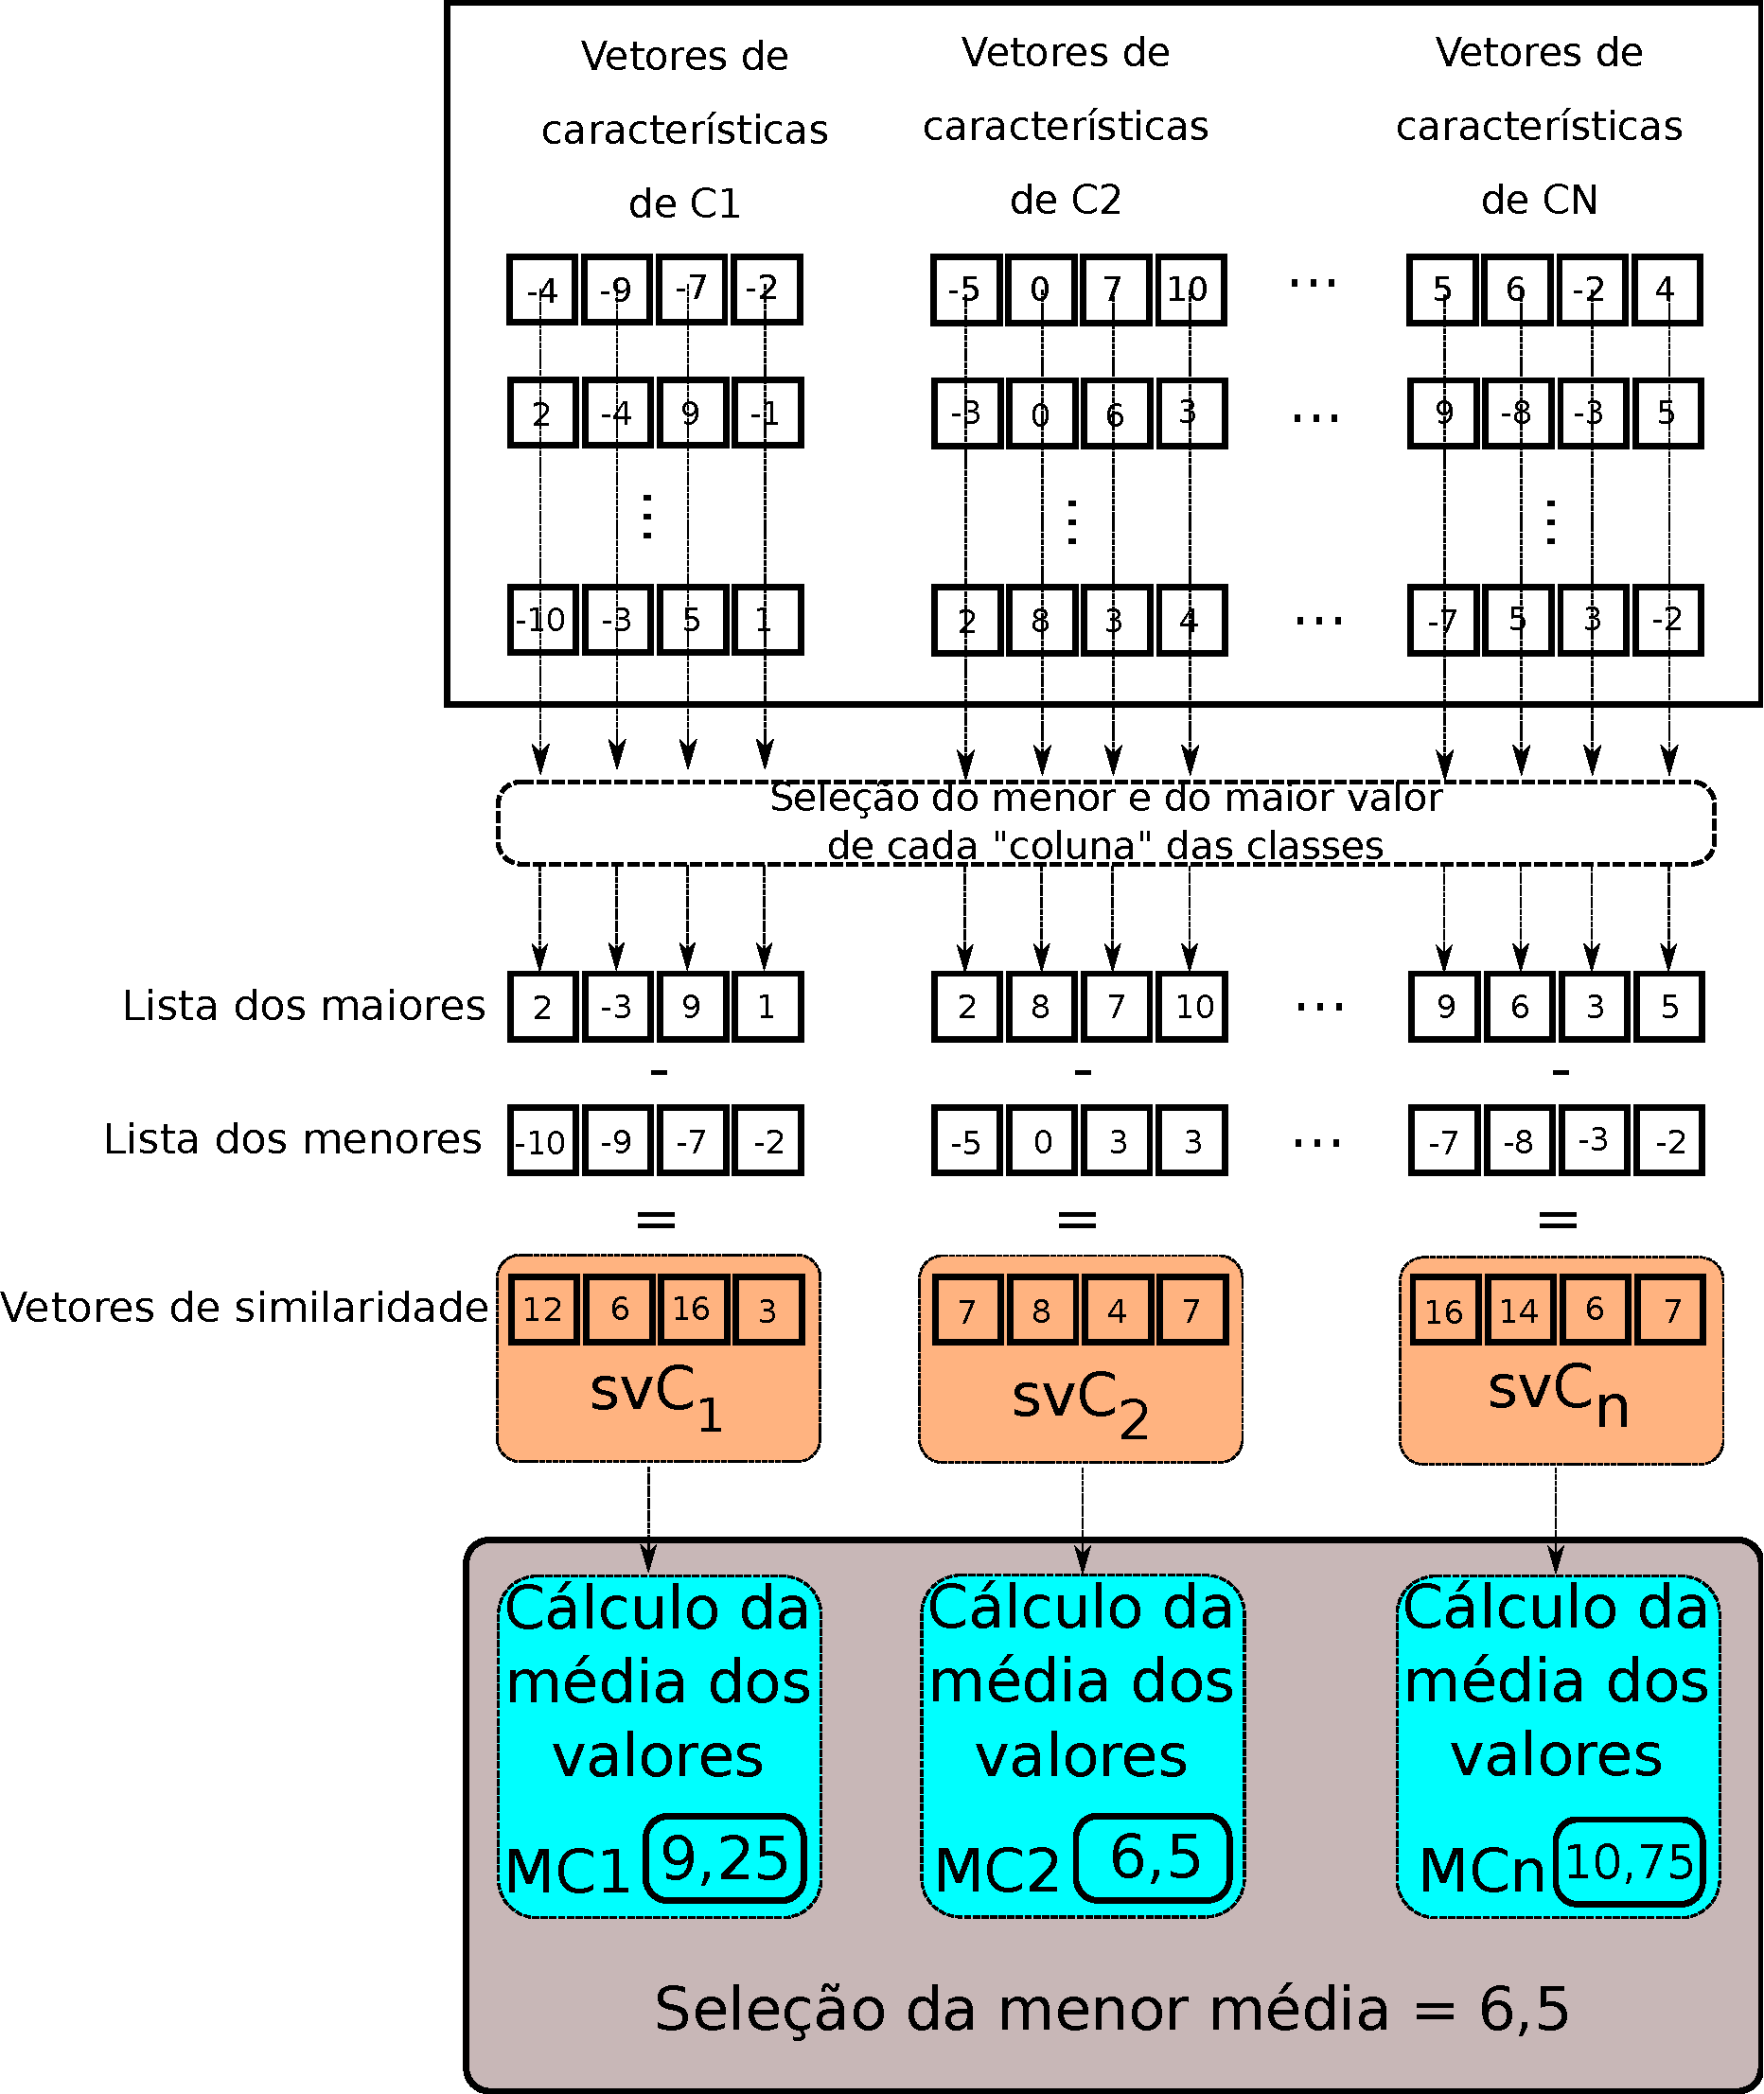
\includegraphics[width=0.77\linewidth]{images/calculoAlpha.pdf}
					\caption{Cálculo do coeficiente $\alpha$.}
					\label{fig:calculoalpha}
				\end{figure}
				
				\par A obtenção de $\beta$, assim como ilustrado na Figura \ref{fig:betacalculation}, também se dá selecionando os maiores e os menores valores de cada uma das posições de todos os vetores de características de cada classe, gerando assim um vetor para os valores maiores e outro para os menores.
				
				\par Na sequência, realiza-se o cálculo de $R$ cujo valor é a quantidade de vezes que um valor do vetor de características de uma classe se encontra entre os valores maiores e menores de outra classe.
				
				\par Seja:
				\begin{itemize}
					\item N a quantidades de classes;
					\item X a quantidade de vetores de características por classe;
					\item T o tamanho do vetor de características.
				\end{itemize}
				
				\par Então, $F$, que é o número máximo de sobreposições possíveis entre classes, é dado por:
				\begin{equation}
						F=N.(N-1).X.T \qquad.
				\end{equation}
				\par Finalmente, $\beta$ é calculado da seguinte forma:
				\begin{equation}
					\beta=\dfrac{R}{F} \qquad.
				\end{equation}
			
				\par Neste ponto, é importante notar que $\alpha=1$ sugere fortemente que os vetores de características de cada classe são similares e representam suas respectivas classes precisamente. Complementarmente, $\beta=0$ sugere os vetores de características de classes diferentes não se sobrepõe \cite{8588433}.
				
				\begin{figure}[h]
					\centering
		    	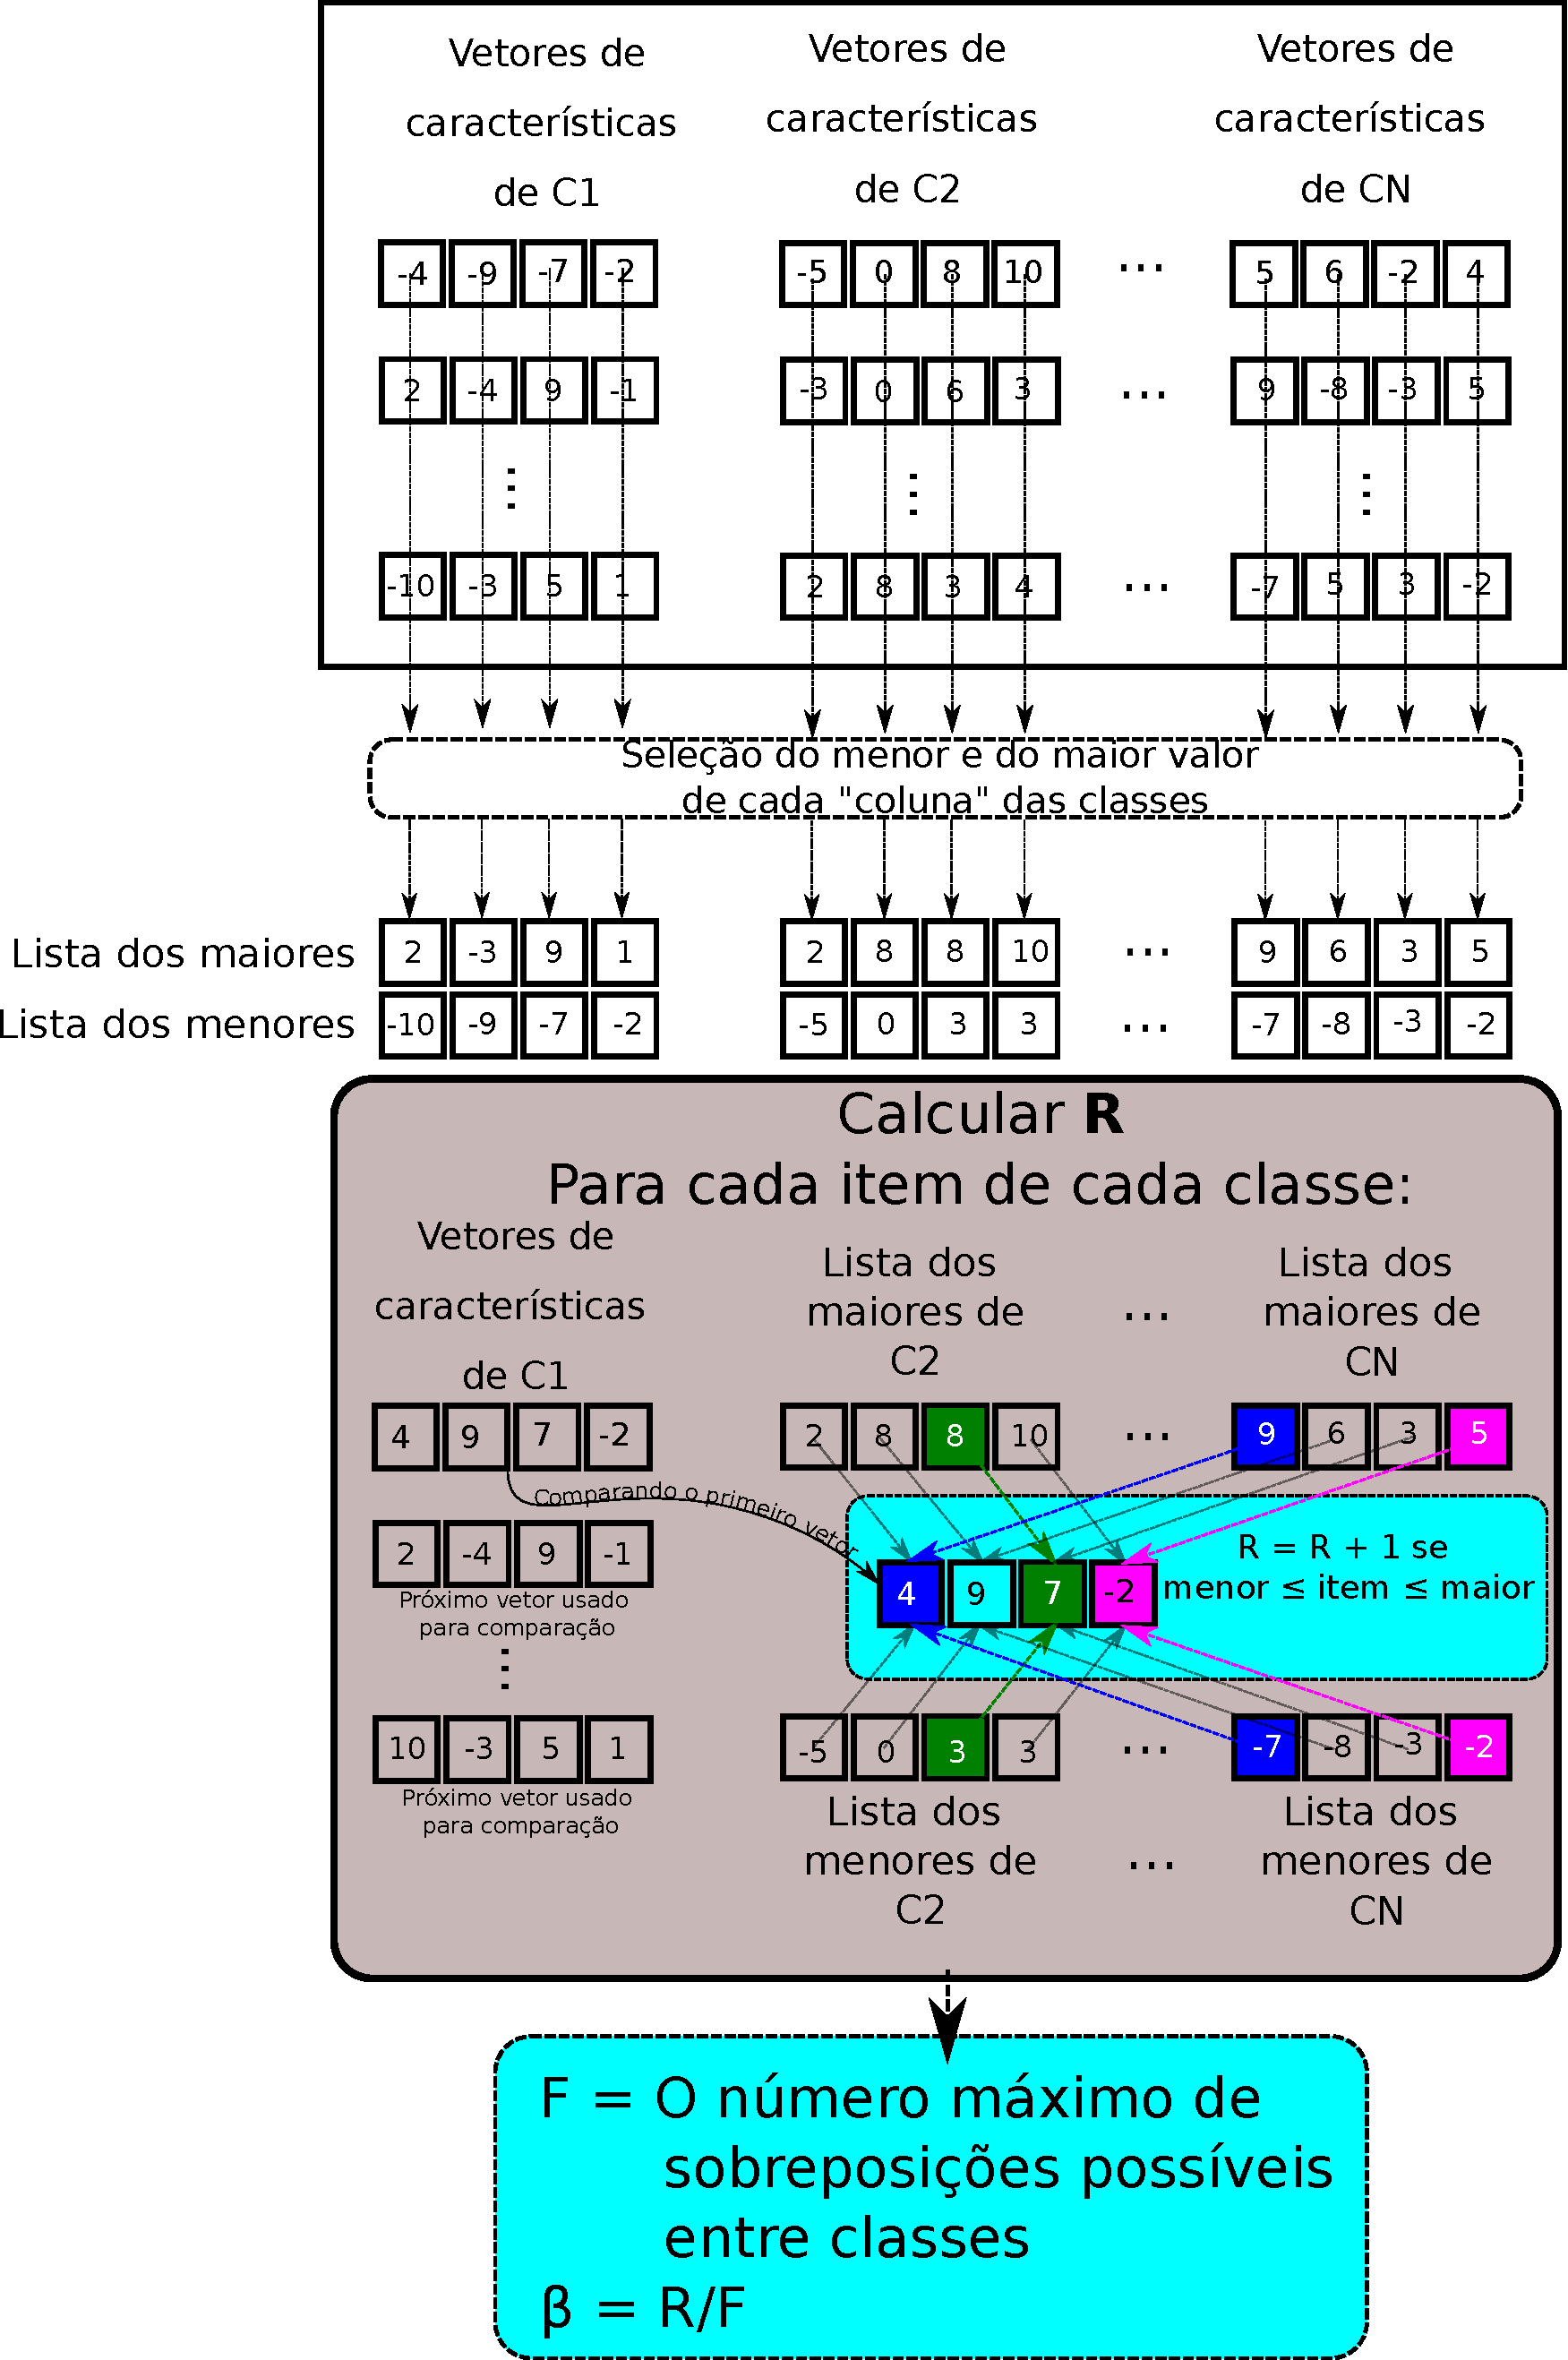
\includegraphics[width=0.77\linewidth]{images/betaCalculation.pdf}
					\caption{Cálculo de $\beta$: Os itens destacados em azul e rosa são aqueles pertencentes a classe C1 e CN que se sobrepõe, em verde, a sobreposição é entre C1 e C2. Para cada sobreposição verificada soma-se 1 ao valor $R$. Essa comparação é feita para todos os vetores de características de cada uma das classes.}
					\label{fig:betacalculation}
				\end{figure}
				\FloatBarrier
			
				\par Considerando-se o plano paraconsistente \cite{8588433}, temos: 
				
				\begin{itemize}
					\item Verdade $\rightarrow$ fé total ($\alpha = 1$) e nenhum descrédito ($\beta = 0$)
					\item Ambiguidade $\rightarrow$ fé total ($\alpha = 1$) e descrédito total ($\beta = 1$)
					\item Falsidade $\rightarrow$ fé nula ($\alpha = 0$) e descrédito total ($\beta = 1$)
					\item Indefinição $\rightarrow$ fé nula ($\alpha = 0$) e nenhum descrédito ($\beta = 0$) \qquad.
				\end{itemize}
				
				\par No entanto, raramente $\alpha$ e $\beta$ terão valores inteiros como os mostrados na listagem acima: Na maioria das ocasiões, $0 \leqslant \alpha \leqslant 1$ e $0 \leqslant \beta \leqslant 1$. Por isso, se torna necessário o cálculo do \textbf{grau de certeza}, isto é, $G_1$, e do \textbf{grau de contradição}, isto é, $G_2$, conforme segue:
				\begin{equation}
					G_1=\alpha-\beta  \qquad,
				\end{equation}
				\begin{equation}
					G_2=\alpha+\beta-1 \qquad,
				\end{equation}
			onde: $-1 \leqslant G_1$ e  $1 \geqslant G_2$.

			\par Os valores de $G_1$ e $G_2$, em conjunto, definem os graus entre verdade ($G_1=1$) e falsidade ($G_1=-1$) e também os graus entre indefinição ($G_2=-1$) e ambiguidade ($G_2=1$). Novamente, raramente tais valores inteiros serão alcançados já que $G_1$ e $G_2$ dependem de $\alpha$ e $\beta$.
		
			\par O Plano Paraconsistente, para fins de visualização e maior rapidez na avaliação dos resultados, encontra-se ilustrado na Figura \ref{fig:paraconsistentplane} e tem quatro arestas precisamente definidas:
			\begin{itemize}
				\item (-1,0) $\rightarrow$ falsidade;
				\item (1,0) $\rightarrow$ verdade;
				\item (0,-1) $\rightarrow$ indefinição;
				\item (0,1) $\rightarrow$ ambiguidade.
			\end{itemize}
			\par A propósito de ilustração na Figura \ref{fig:paraconsistentplane}, é possível ver um pequeno círculo indicando os graus dos quatro casos listados.
	
			\par Para se ter ideia em que área exatamente se encontram as classes avaliadas, as distâncias $(D)$ do ponto $P=(G_1,G_2)$ até o limites supracitados podem ser computadas. Tais cálculos podem ser feitos da seguinte forma:

			\begin{equation}
				D_{-1,0}=\sqrt{(G_1+1)^2+(G_2)^2}\qquad,
			\end{equation}
			\begin{equation}
				D_{1,0}=\sqrt{(G_1-1)^2+(G_2)^2}\qquad,
			\end{equation}
			\begin{equation}
				D_{0,-1}=\sqrt{(G_1)^2+(G_2+1)^2}\qquad,		
			\end{equation}
			\begin{equation}
				D_{0,1}=\sqrt{(G_1)^2+(G_2-1)^2}\qquad.
			\end{equation}		

			\begin{figure}[h]
				\centering
				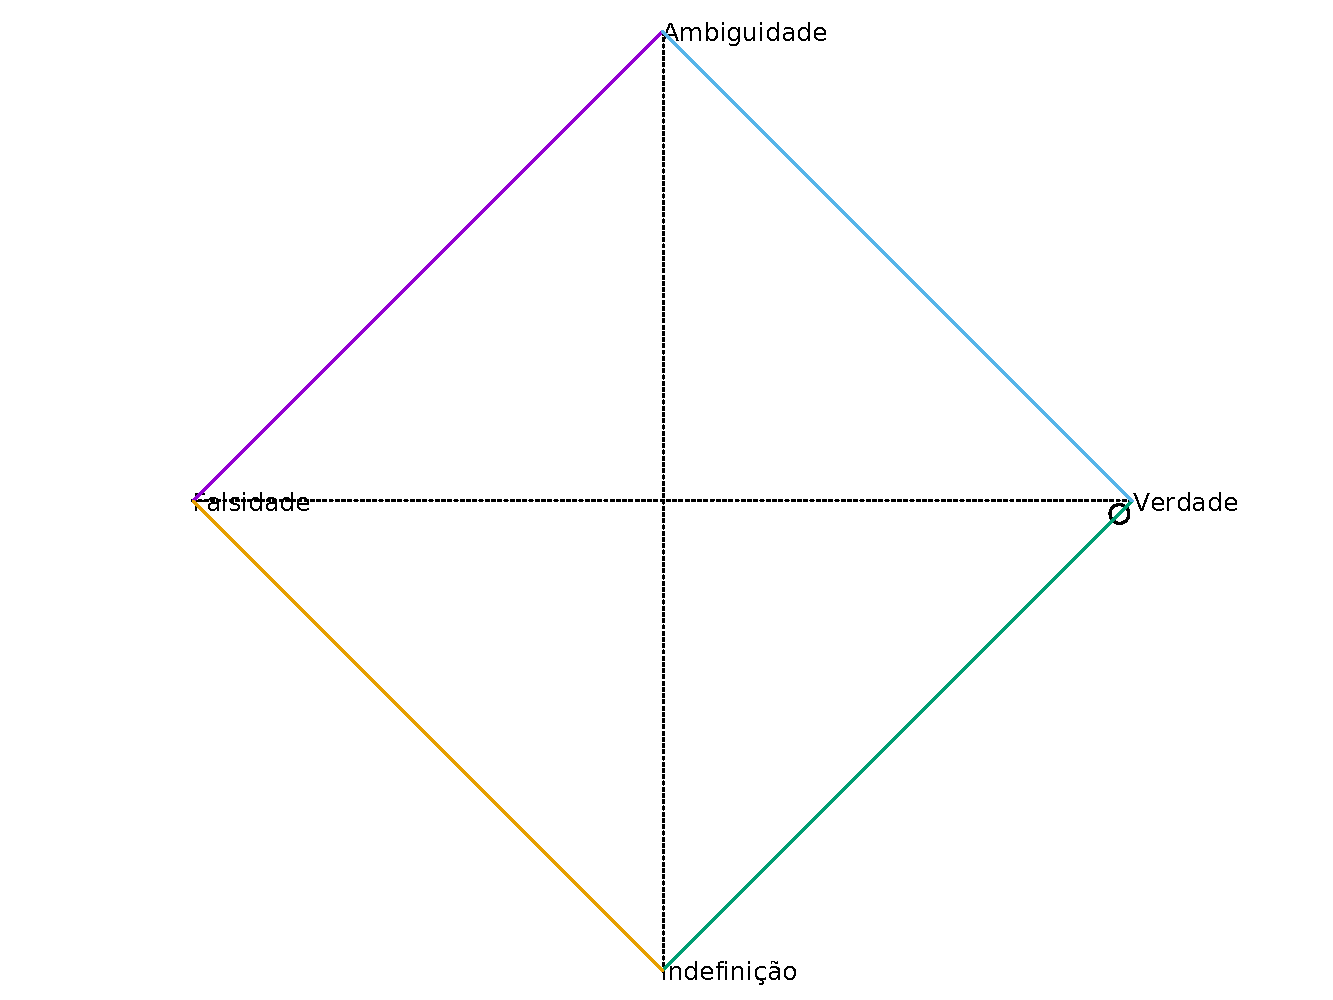
\includegraphics[angle=-90, width=0.69\linewidth]{images/paraconsistentPlane.pdf}
				\caption{O plano paraconsistente: O pequeno círculo indica os graus de falsidade(-1,0), verdade(1,0), indefinição(0,-1) e ambiguidade(0,1)}
				\label{fig:paraconsistentplane}
			\end{figure}
		
		\par Na prática, ou seja, para fins de classificação, geralmente considera-se a distância em relação ao ponto \textit{``(1,0) $\rightarrow$ Verdade''}, que é o ponto ótimo: quanto mais próximo o ponto $(G_1,G_2)$ estiver de $(1,0)$, mais as os vetores de características das diferentes classes estão naturalmente separados. Isso implica a possibilidade do uso de classificadores mais modestos. 
		
	\section{Estado-da-arte em \textit{Playback Speech Detection}}
		\par No artigo \citetext{Ren2019} foi apresentado um esquema de diferenciação entre a fala comum e aquela vinda de um dispositivo reprodutor. O foco da análise se deu na distorção causada pelo alto-falante, segundo a energia e outras várias características do espectro do sinal. Uma base com 771 sinais de fala foi criada para cada um dos quatro dispositivos de gravação usados, totalizando 3084 segmentos de voz. Uma SVM foi usada como classificador. De acordo com os experimentos, a \textit{taxa de verdadeiros positivos} foi de 98,75\% e a \textit{taxa de verdadeiros negativos} foi de 98,75\%.\\
		
		\par Em \citetext{DiqunYan2019} é mostrado um método para diferenciar a voz de um locutor verdadeiro da voz gerada por sistemas usando sintetizadores baseados no \textit{modelo oculto de Markov} (HMM). SAS 2019\cite{SAS2019} foi a escolha de base de dados. Este método usa coeficientes de características logarítmicos extraídos de wavelets que são apresentados a um classificador SVM. Os resultados obtidos tiverem, em média, mais de 99\% de acurácia.\\

		\par Usando uma decomposição por espalhamento baseada em \textit{wavelets} e convertendo o resultado em coeficientes cepstrais (SCCs), o artigo \citetext{7802552} contém a descrição de um vetor de características que é avaliado por Modelos de Misturas Gaussianas (GMM) para fins de \textit{playback speech detection}. SAS 2015 \cite{SAS2015} foram as bases de dados escolhidas para os testes. Em relação aos resultados, foram usadas a \textit{taxa de falsos verdadeiros} (FAR) que representa a taxa de ocorrências falsas classificadas como verdadeiras e a \textit{taxa de falsos falsos} (FRR) que é a taxa de ocorrências verdadeiras classificadas como falsas. Os pontos em que FAR é igual a FRR foram definidos como pontos de taxa de erros iguais (ERR) e a relação $\dfrac{FAR}{FRR}$, igual a 0,18 naquele caso, foi usada como parâmetro de avaliação.\\

		\par Em \citetext{alluri2019replay}, os autores usam o \textit{zero time windowing} ou janelamento de tempo zero (ZTW) para, em conjunto com a análise cepstral do espectro gerado, fazer a análise dos sinais de voz. Os experimentos foram feitos usando-se a base SAS 2017\cite{SAS2017} com um classificador GMM e a taxa geral de ERR dos experimentos foi de 0,1475.\\
		
		\par Em \citetext{8725688}, foi registrado uma diferença entre as propriedades espectrais da voz original e da voz gravada, que pode ser expressa por meio de coeficientes cepstrais. Um GMM foi usado como classificador e a base de dados usada foi a SAS 2017. Quanto aos resultados, foi obtida uma EER geral menor que 0,1.\\
	
		\par A proposta do artigo \citetext{Hanilci2018} foi usar sinais residuais de predição linear para, juntamente com coeficientes cepstrais, criar características que foram apresentas a um classificador GMM. Novamente, a base de dados usada foi a SAS 2015 e os resultados em ERR geral foram de 5,249.\\

		\par Para detecção de \textit{playback speech}, os autores do artigo  \citetext{ISI:000473343500086} importaram, da área de processamento de imagens, o conceito de textura para o processamento de voz. Padrões binários locais (LBP) e seus respectivos histogramas foram usados para a construção do vetor de características que foi avaliado por uma SVM. A base de dados usada para testes foi a SAS 2015 e a taxa máxima de acurácia conseguida foi de 0,7167.\\
		
		\par Uma abordagem que combina análise de sinal de fala usando a \textit{Transformada Constante Q} (CQT) com o processamento cepstral foi mostrada no artigo \citetext{TODISCO2017516}. Essa técnica resulta no que se chama \textit{Coeficientes Cepstrais de Constante Q}(CQCCs). Segundo o artigo, a vantagem desses coeficientes é a resolução de espectro temporal variável. As bases de dados usadas foram a RedDots \cite{redDots}, SAS 2015 e AVSpoof 2015 \cite{AVSpoof2015}. Em se tratando de classificadores foram usados dois GMMs, cada um treinado usando os dados genuínos e \textit{spoofing} respectivamente. Os testes realizados para cada uma das bases chegou aos seguintes resultados: SAS 2015 $\rightarrow$ EER geral de 0.026; AVSpoof 2015 $\rightarrow$ EER geral de 0; RedDots $\rightarrow$ EER geral de 0,185.\\

		\par No artigo \citetext{Patel2015} é usada a \textit{Transformação Auditiva (TU)}, que tem como base a transformada \textit{wavelet}, e a \textit{Cochlear Filter Cepstral Coefficients (CFCC)} que é a junção dos métodos citados mais uma média dos valores em um intervalo de janela definido. Além disso, se define a \textit{estimação da frequência instantânea (IF)} que tem por base a Transformada de Hilbert \cite{johansson1999hilbert} e \cite{kschischang2006hilbert}. O processo todo tem como objetivo emular mecanismos naturais ocorridos dentro do ouvido e usa, além da \textit{TU}, o cálculo de coeficientes cepstrais e transformada cosseno. Para a composição dos vetores de características foram combinadas as técnicas \textit{MFCC}, \textit{CFCC}, \textit{CFCC+IF}. A base de dados usada foi a AVSpoof 2015. O classificador utilizado foi um GMM, as classificações chegaram uma EER de 0.083.\\

		\par O artigo \citetext{ISI:000490497200068} propõe uma solução para distinguir sinais de voz genuínos daqueles falseados usando reverberação e as partes não vozeadas da fala. Três GMMs foram definidos para a classificação, nesta estratégia os mesmos votam se uma ocorrência é ou não verdadeira, ganhado sempre a classificação que obtiver mais votos. A base de dados utilizada foi a  fornecida pelo \textit{``Automatic  Speaker Verification and Spoofing Contermeasures Challenge 2017''}(ASVSpoof 2017). O sistema de avaliação de desempenho escolhido, novamente, foi a ERR e esta alcançou um valor de 2,99.\\
		
		\par A principal ideia do artigo \citetext{ISI:000465363900136} foi a de capturar a amplitude instantânea vinda de flutuações de energia para distinguir entre sinais de voz genuínos daqueles falseados. Segundo os autores, as modulações de amplitude são mais suscetíveis ao ruído inserido no sinal original por uma fonte reprodutora. O estudo usa a base de dados fornecida pelo ASVSpoof 2017 e GMM como classificador. Os resultados apresentados chegaram a uma EER de 0.0019.\\

		\par No trabalho \citetext{ISI:000465363900139}, foram usadas as diferenças entre bandas de frequências específicas para diferenciar um sinal legítimo de um usado em ataques de falsificação. Particularmente, foi proposta a \textit{predição linear em domínio de frequência}(FDLP) juntamente com GMMs para classificação dos dados presentes na base  fornecida pelo ASVspoof  2017. Os resultados apresentados implicam a EER de 0.0803.\\
		
		\par No artigo \citetext{Suthokumar2018}, os autores propuseram duas novas características que visam interpretar as componentes estáticas e dinâmicas do sinal, complementando as características de tempo restrito no espectro, para distinguir entre locuções genuínas e regravadas. São elas a \textit{Modulation  Spectral Centroid Frequency} e \textit{Long Term Spectral Average}. O sistema usa como classificador um GMM juntamente com a base dados fornecida pelo ASVSpoof 2017. Os resultados mostram um valor de EER de 0,0654.\\
		
		\par Considerando o envelopamento das amplitudes e  frequências instantâneas em cada banda estreita filtrada, os autores do artigo \citetext{ISI:000458728700054} discutiram como diferenciar um sinal de voz legítimo de um falseado. A base de dados usada foi a fornecida pelo \textit{``Automatic  Speaker Verification and Spoofing Contermeasures Challenge 2015''} (ASVSpoof 2015) e o GMM foi o classificador escolhido. A proposta alcançou a EER de 0,045.\\

		\par No artigo científico \citetext{ISI:000392503100008}, foi proposto o uso do \textit{gammatone frequency cepstral coefficients}(MGFCC). O gammatone é o produto de uma distribuição gamma com um sinal senoidal e é usado na construção de filtros auditivos que, neste caso, são usados para extrair características do sinal de voz. A base de dados usada foi a fornecida pelo ASVspoof 2015 e o classificador usado foi um GMM. Na distinção entre vozes genuínas e regravadas, o EER chegou a 0,02556.\\
		
		\par Segundo o artigo \citetext{8396208}, o \textit{hashing} sensível a \textit{locus} (LSH), que é frequentemente usado como um classificador para problemas relacionados a \textit{big data}, foi combinado com coeficientes MFCCs para distinção entre locuções genuínas e regravadas. No método, os MFCCs foram extraídos dos arquivos de sinal para posterior aplicação do LSH, gerando assim uma tabela \textit{hash}. Esses valores de \textit{hash} foram então comparados, identificando assim o locutor ou locutora. Nos testes realizados houve uma acurácia de 92,66\%, a base de dados usada foi a TIMIT 2018 \cite{TIMIT2018}. \\

		\par Apesar do uso de \textit{wavelets} em alguns artigos \cite{DiqunYan2019}, \cite{Patel2015}, \cite{7802552} é interessante notar, pelo menos até o presente momento, que seu uso é escasso em técnicas de prevenção de \textit{voice spoofing}. Em uma das abordagens mais originais que usa as partes não vozeadas do sinal \cite{ISI:000490497200068}, seria muito útil o uso das transformadas \textit{wavelet} ou \textit{wavelet packet}. Tanto neste documento como em boa parte das referências utilizadas, é comum o uso de uma escala \textit{MEL} combinada com outras técnicas para construção do método de detecção de \textit{voice spoofing} \cite{Hanilci2018}, \cite{Patel2015}, \cite{8396208}, \cite{8725688}, \cite{ISI:000490497200068}. No entanto, em nenhuma dessas publicações se utilizou a escala \textit{BARK}, que foi, surpreendentemente, a que demonstrou  os melhores resultados no caso específico desta dissertação. O uso de coeficientes cepstrais combinados com outras técnicas foi muito comum \cite{alluri2019replay}, \cite{7802552}, \cite{8725688}, \cite{Hanilci2018}, \cite{TODISCO2017516}, \cite{Patel2015}, \cite{ISI:000392503100008}. Escolhidos os métodos de geração dos vetores de características, foram selecionados classificadores variados, com destaque para o relativamente simples \textit{Gaussian Mixture Models}(GMM), o mais escolhido. Este trabalho também contou com a escolha de dois classificadores modestos: Por distância Euclidiana / Manhattam e Máquina de Vetores de Suporte.\\
		
		\par A leitura dos artigos mencionados nesta seção indica ainda que, aparentemente, dentro do contexto de \textit{voice spoofing}, o esforço é para se criar vetores de características cada vez melhores, sendo curioso que em nenhum dos escritos consultados houvesse uma metodologia para comparação de resultados que não fosse a manual. Nesta dissertação, existe uma série de métodos candidatos para geração dos vetores de características baseados em \textit{wavelets} e nas escalas \textit{BARK} e \textit{MEL}. Tais candidaturas foram avaliadas segundo a engenharia paraconsistente de características que selecionou a melhor combinação dentre as opções apresentadas. Em se tratando de resultados, a maioria dos trabalhos, devido ao uso das bases \textit{SAS} e \textit{AVSpoof}, apresentaram seus resultados segundo a \textit{Equal Error Rate (EER)} que é a medida padrão para avaliação. Alguns outros utilizaram somente a acurácia \cite{8396208}, \cite{ISI:000473343500086}, \cite{DiqunYan2019}, \cite{Ren2019} e medidas calculadas em tabelas de confusão. Neste trabalho, todas as referidas métricas foram consideradas.\\
